\section{Introduction}

In this section, we will look at the structure of Sun and then proceed to eruptive events like Solar flares, Coronal Mass Ejections, Stellar Coronal Mass Ejections, Coronal Dimming.

\subsection{Sun}

The Sun is a conspicuous and important celestial body that provides Earth with its
primary heat, light, and energy supply as well as acting as the gravitational anchor for our
solar system. It is a yellow dwarf, or G-type main-sequence star, that is located at the heart
of our solar system. Knowing the Sun is essential to understanding the dynamics of our
planetary system, as well as to obtain knowledge of basic astrophysical processes and the
properties of stars in the larger universe. Sun is a massive object that makes up around
99.86\% of the solar system’s total mass. With a diameter of roughly 1.4 million kilometers,
it is roughly 109 times bigger than Earth. In comparison to the enormous diversity of stars
in the cosmos, the Sun is regarded as an average-sized star despite its enormous size.\\

Sun is an essential component of keeping life on Earth alive. Its emission of energy
affects weather patterns, ocean currents, and ecosystems, driving the planet’s climate. Pho-
tosynthesis, the process by which plants turn carbon dioxide into oxygen and build the base
of the food chain, is made easier by sunlight. The steady orbits of planets in our solar system
are also maintained by the gravitational pull of the Sun.\\

Our knowledge of the Sun has greatly increased because to scientific tools and satellite
missions like the Solar and Heliospheric Observatory (SOHO), the Solar Dynamics Obser-
vatory (SDO), and most recently, Aditya-L1. With the use of these instruments, scientists
are able to track solar activity, detect solar phenomena, and investigate the Sun’s effects on
the solar system and beyond.

\subsection{Structure of the Sun}

Sun is divided into three regions, namely, interior region, visible surface and atmosphere. The interior region is further divided into core, radiative zone and convective zone. The \textbf{core} is the main fuel station for Sun, where nuclear fusion process is converting H to He. The radiations produced during the fusion process escapes through the surface as visible light. The \textbf{radiative zone} extends from the outer edge of the core to the base of the convective zone. \Cref{fig:structure_of_sun} shows the structure of Sun. The layer that separates the Sun's interior and it's atmosphere is called as \textbf{photosphere}. The outer atmosphere of the Sun is called the \textbf{corona}, which is a source of solar wind. The inner atmosphere of the Sun is known as the \textbf{chromosphere}. Because of the high hydrogen content, Sun appears red when viewed through a solar telescope, hence the name chromosphere.

\begin{figure}[h!]
    \centering
    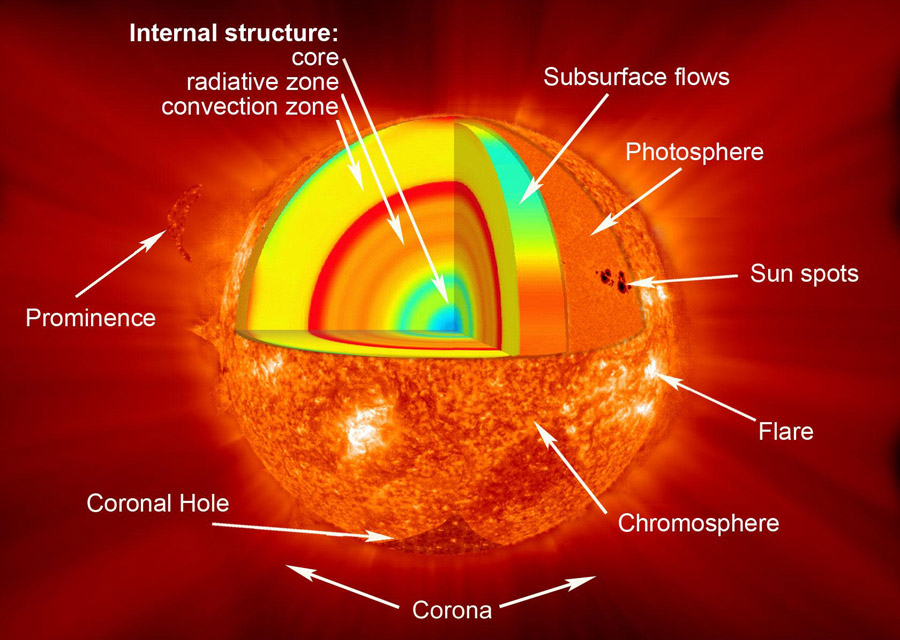
\includegraphics[width=0.5\textwidth]{images/structure_of_sun.jpg}
    \caption[Structure of the Sun]{Structure of Sun. (Image credit: NASA)}
    \label{fig:structure_of_sun}
\end{figure}

The radiations produced in the core radiates slowly outwards through this region into the convective zone, taking more than about 170,000 years to radiate through this layer. The \textbf{convective zone} is the region where the plasma, through the process of convection currents of heated and cooled gas, moves towards the surface.

\subsection{Solar Corona}

Outermost layer of the Sun's atmosphere is known as Solar Corona. It lies above the chromosphere and extends millions of kilometers into outer space. Corona can be easily viewed during solar eclipse (\cref{fig:corona_eclipse}), but can also be observed using a coronagraph. Coronagraph is a device that occults the disk of the Sun (similar to how moon occults the Sun during solar eclipse) thereby enabling easy coronal observations and analysis.

\begin{figure}[h!]
    \centering
    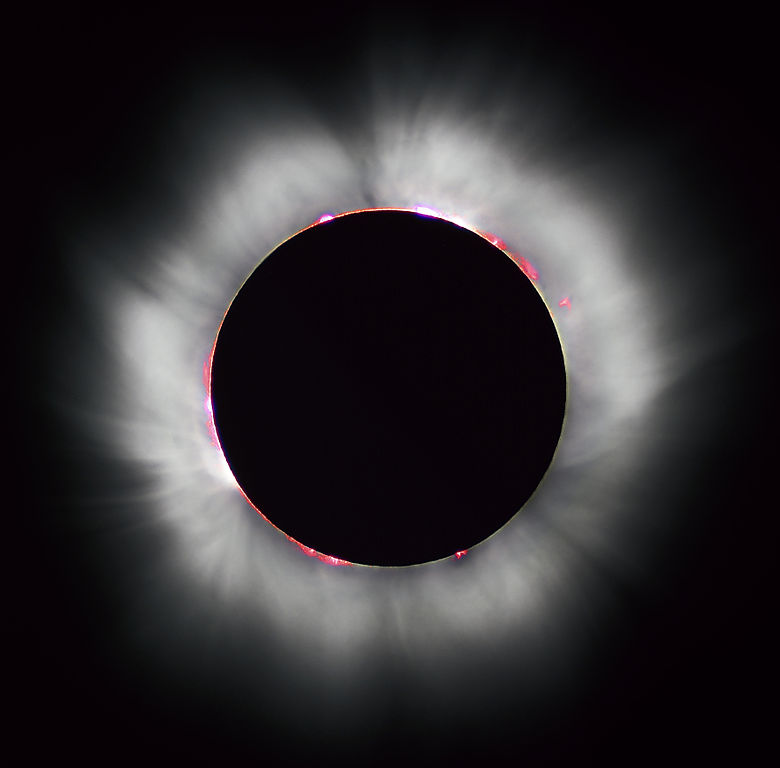
\includegraphics[width=0.5\textwidth]{images/corona.jpg}
    \caption[Image of Solar corona during a total solar eclipse]{Image of Solar corona during a total solar eclipse. (Image credit: NASA)}
    \label{fig:corona_eclipse}
\end{figure}

The temperature of solar corona is of the order of million of degree kelvin. The emitted plasma can been seen in the EUV region and it is possible to observe the corona using EUV filters without a coronagraph. The unusual spectral features of the solar corona have been explained by the existence of Fe XIV (or Fe$^{13+}$). \citep{aschwanden2006physics}

\subsection{Solar Flares}

Explosive phenomenas that occur on the surface of sun are called as solar flares, caused by the reconnection of a sun's magnetic field lines. These flares are often accompanied by filaments/prominent eruptions and Coronal Mass Ejections (CMEs). Flares are classified into two types: \textit{eruptive} and \textit{confined}. Eruptive events are the flares which are associated with CMEs and confined flares are those which are not associated with CMEs. Plasma and magnetic field structures sometimes extend outwards from the surface. These structures are called filaments/prominences. Filaments and prominences are fundamentally of the same physical properties, only difference is the angle at which it is observed. If plasma floats outside the solar limb, it is called prominence, it is called a filament if it is within the solar background otherwise \cref{fig:filament_prominence}. Difference is in the type of spectrum obtained, which is Balmer lines in emission spectra in case of prominences and absorption lines in case of filaments. Loop-like structures of plasma stand out brightly against the dark background of space, these are prominences. An image of solar flare event of \nth{4} August 2011 is shown in \cref{fig:solar_flare_4_aug_2011}.

\begin{figure}
    \centering
    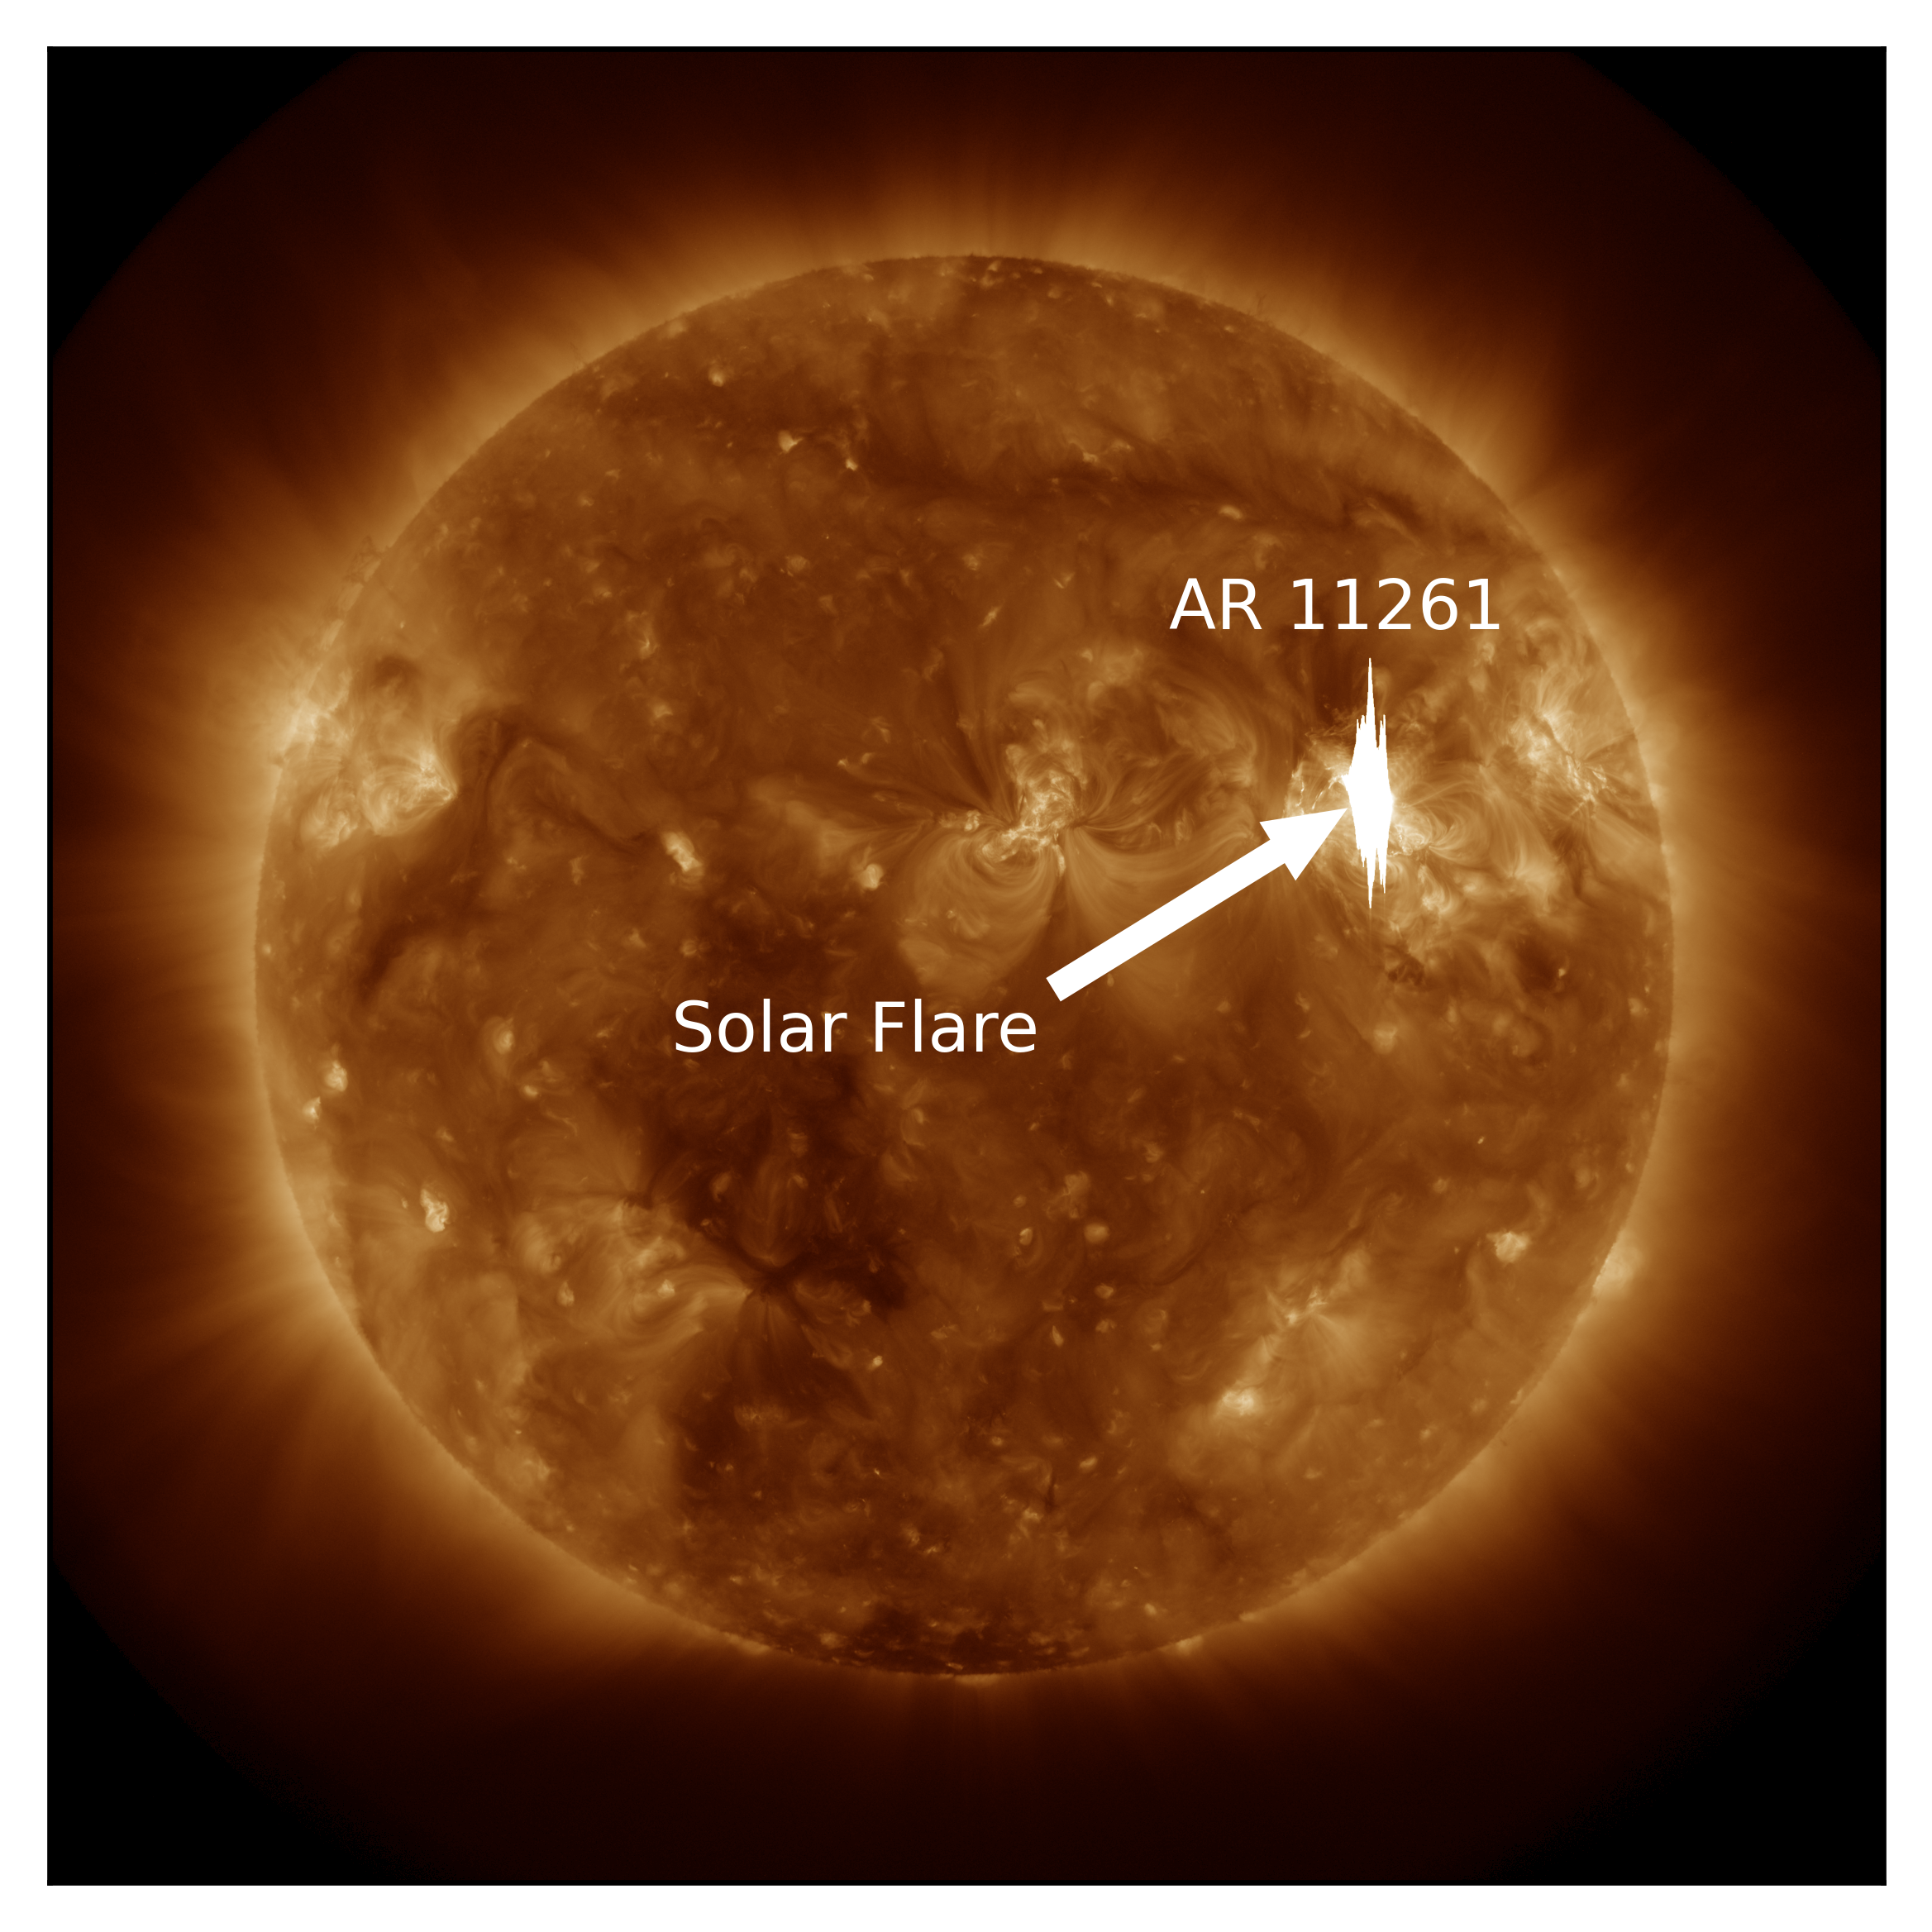
\includegraphics[width=0.5\textwidth]{images/solar_flare_4_aug_2011.png}
    \caption[Solar flare (\nth{4} August 2011)]{Solar flare event of \nth{4} August 2011 originating from the Active Region AR 11261 observed through 193 \AA \ AIA channel}
    \label{fig:solar_flare_4_aug_2011}
\end{figure}

\begin{figure}
     \begin{subfigure}[b]{0.5\textwidth}
         \centering
         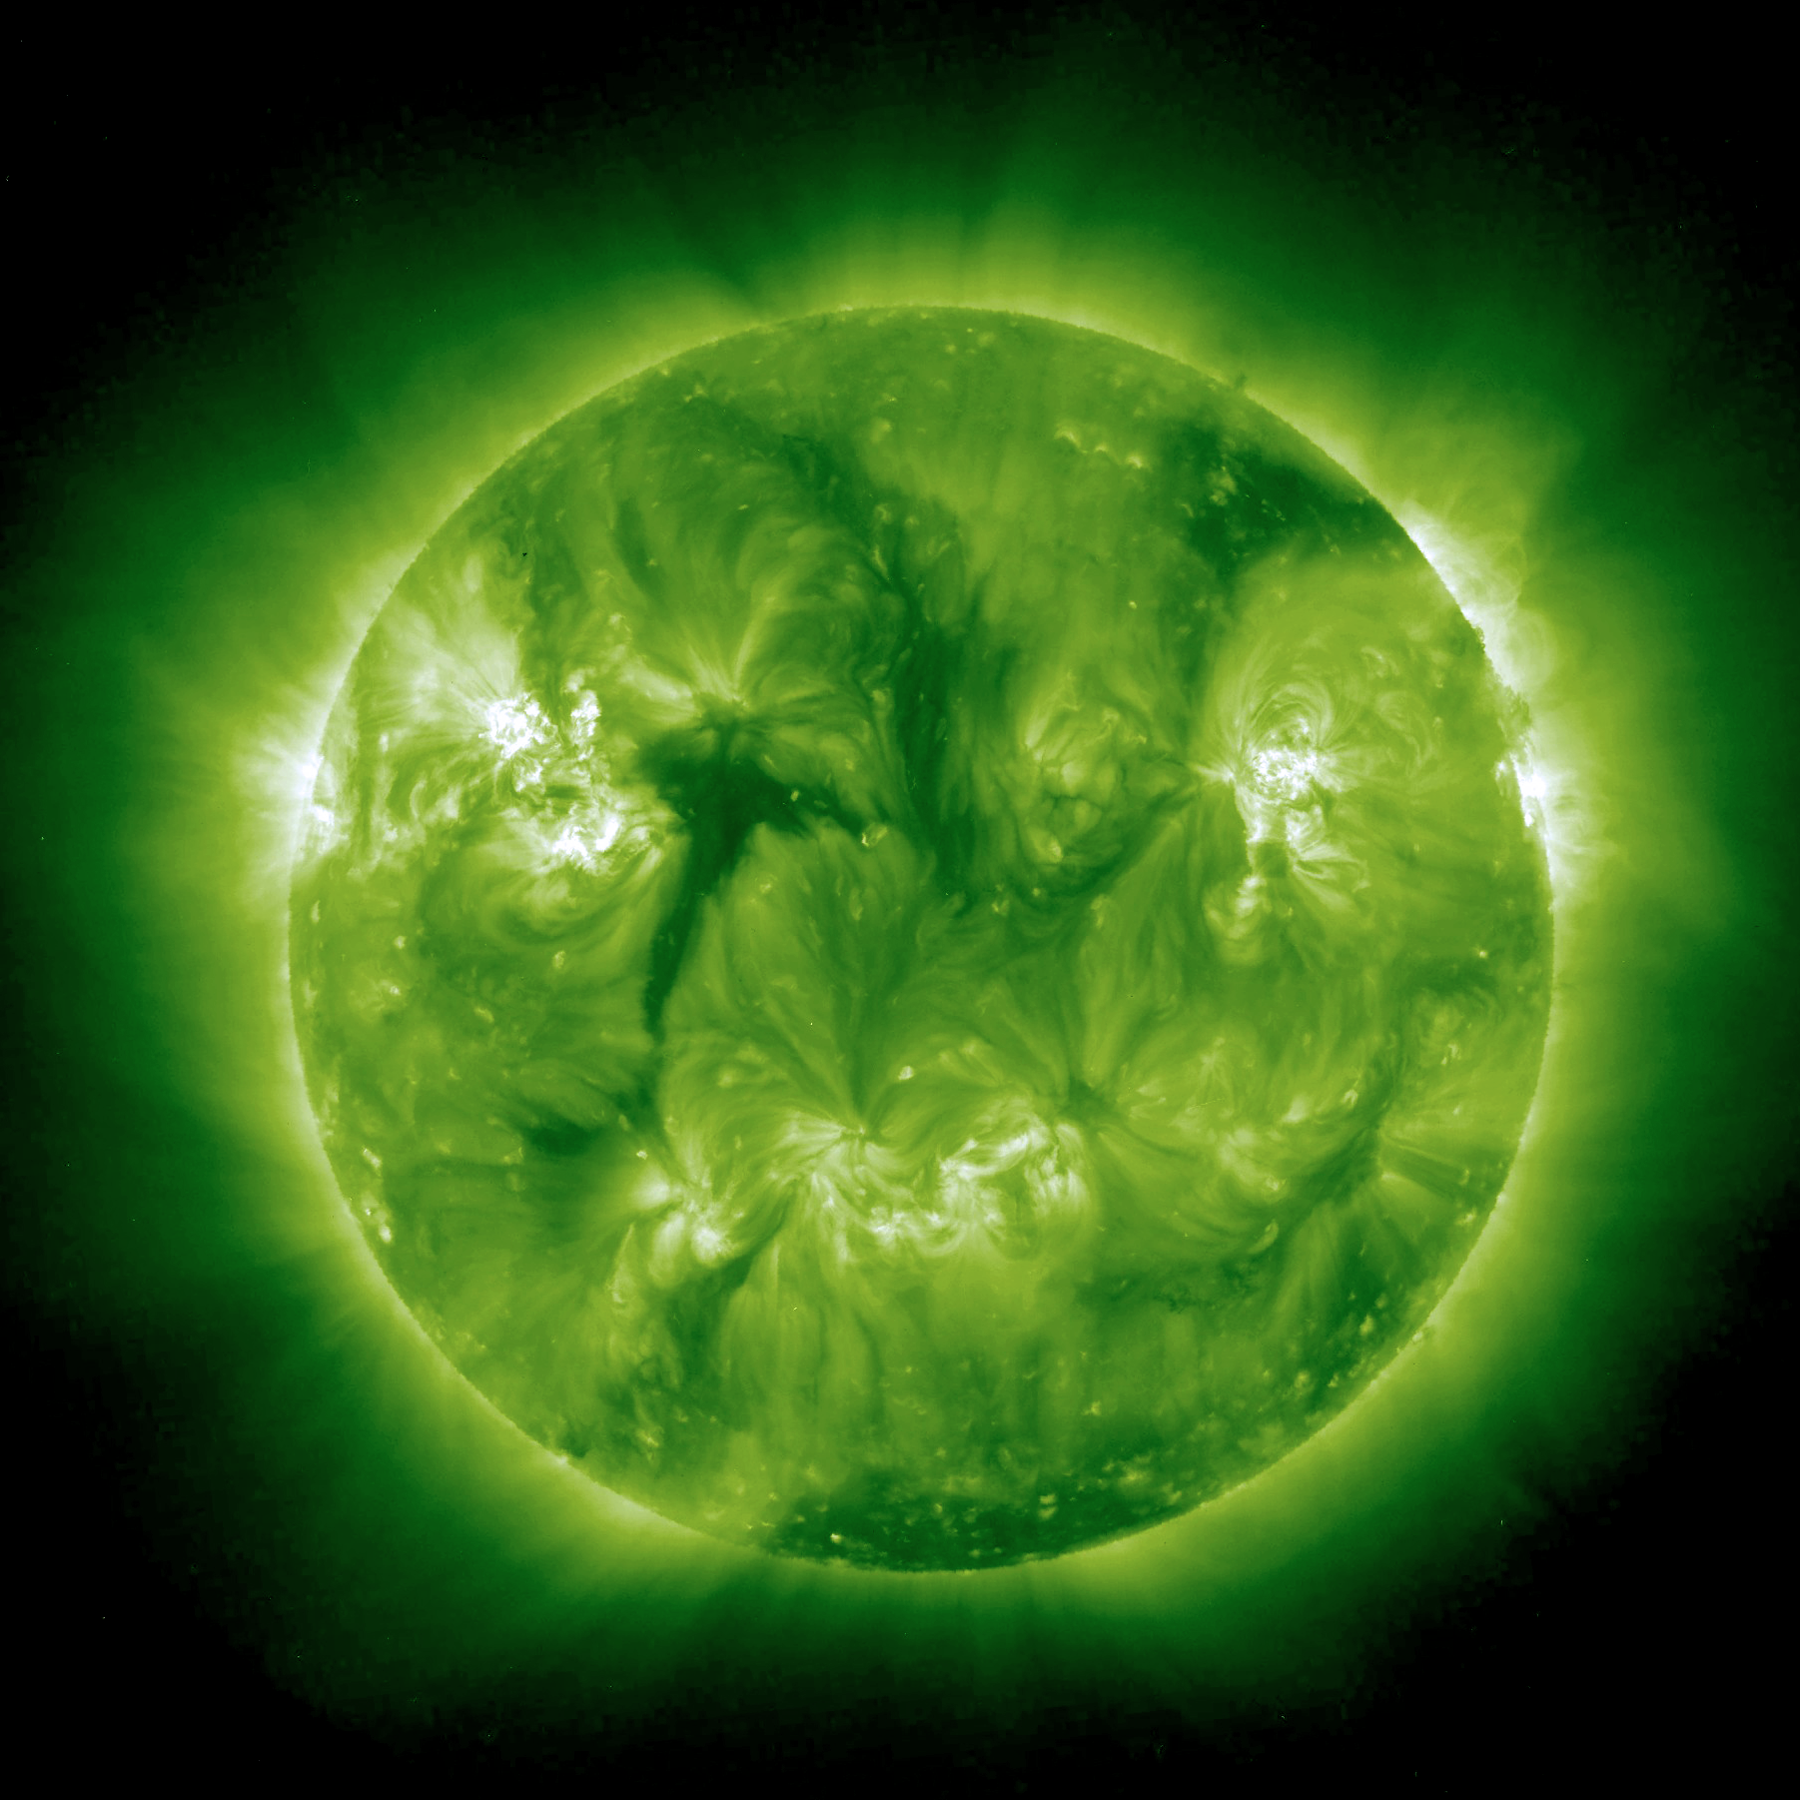
\includegraphics[width=\textwidth]{images/195_Filament.png}
         \caption{Filament}
         \label{fig:filament}
     \end{subfigure}
     \hfill
     \begin{subfigure}[b]{0.5\textwidth}
         \centering
         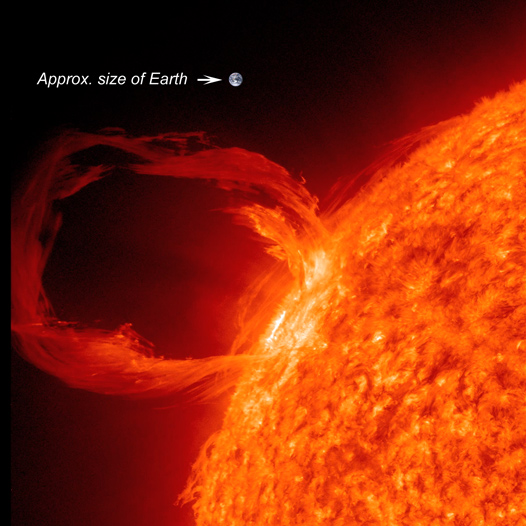
\includegraphics[width=\textwidth]{images/prominence.jpg}
         \caption{Prominence}
         \label{fig:prominence}
     \end{subfigure}
     \caption[Filament and Prominence]{\Cref{fig:filament} shows a U-shaped very long filament which was stable for a period of two days (\nth{6} - \nth{7} February 2012) . \Cref{fig:prominence} is a prominence eruption seen in Extreme UV light on \nth{30} March 2010 (credit: NASA).}
     \label{fig:filament_prominence}
\end{figure}

\subsection{Coronal Mass Ejections (CMEs)}

CMEs are large plasma structures ejected from the solar surface to the heliosphere. They were first discovered in 1971 \citep{Gopalswamy2016-nm}. They majorly affect the space weather, causes interplanetary disturbances and shock waves. CMEs propagting towards the earth can disrupt the communication technologies like satellites. Filament eruptions and solar flares are often associated with CMEs. These energetic plasma have energy of the order of $10^{29} - 10^{32}$ erg and fast speeds even up to 3600 $kms^{-1}$

\subsection{Stellar CMEs}

Similar to solar flares, stellar flares maybe associated with CMEs, but it is not easy to detect or study them as there is no spatial resolution unlike Sun. CMEs accompanied by stellar flares are substantially larger in comparison to the ones observed on the Sun, and have been known to affect the exoplanets around the host stars \citep{Veronig2021-rf}. Hence studying the CMEs is very crucial for future exoplanetary expeditions also. Indirect stellar CME detections have been explored with methods such as coronal dimming, blueshifted emission of chromospheric lines, X-ray, EUV and FUV dimming, Type-II and type-IV radio bursts etc \citep{Korhonen2016-jo}. Conceptually, stellar CMEs energetics might be thought of as an extrapolation of case of solar CME. But, \citep{Argiroffi2019} found that the ratio of stellar CMEs to the flaring energy is not found to be extrapolated version of solar case as seen in \cref{fig:stellar_cme_energy_mass_relation}.

\begin{figure}[ht]
    \centering
    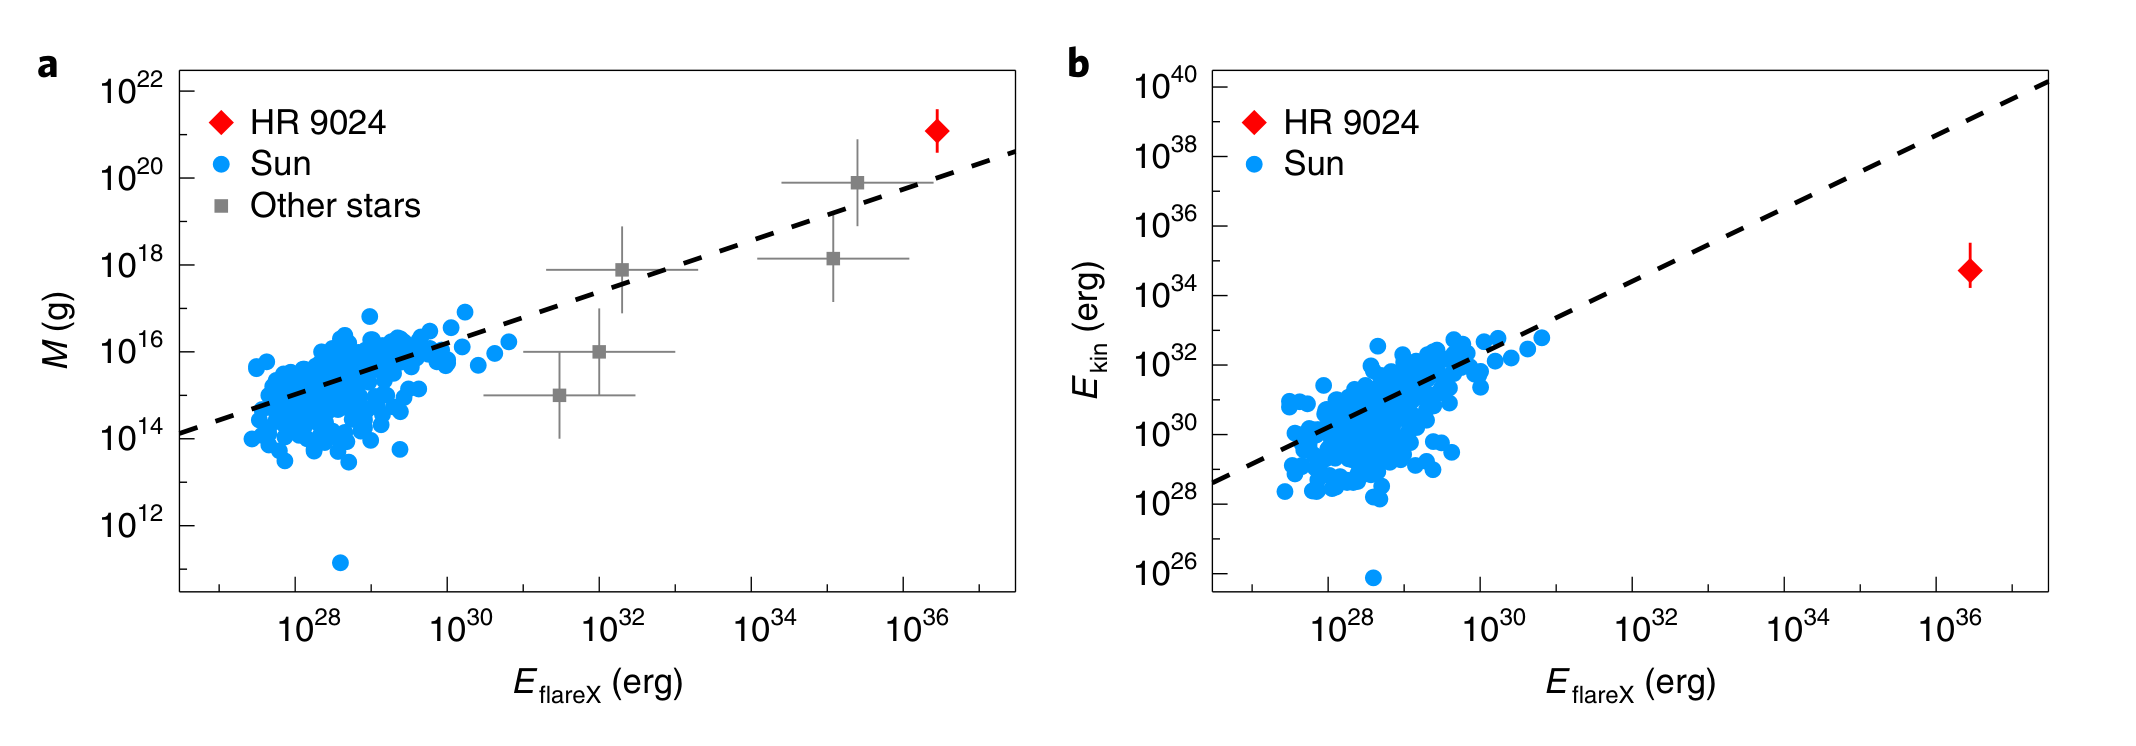
\includegraphics[width=\textwidth]{images/stellar_cme_energy_mass_relation.png}
    \caption[Extrapolation of Solar flare-CME relation]{Extrapolation of the solar flare-CME relation. Mass and kinetic energy of solar CMEs shown as a function of X-ray fluence of the associated flares. \capcite{Argiroffi2019}}
    \label{fig:stellar_cme_energy_mass_relation}
\end{figure}


\subsection{Coronal Dimming}

Coronal dimming is considered one of the promising signatures to detect the occurence of stellar CMEs \citep{Namekata2022-dm}. Regions with temporary dimming of plasma on the solar surface is seen after an eruptive event like CMEs in the EUV and soft X-ray wavelengths. This dimming observed is due to the mass loss in the corona after an eruptive event like CME \citep{Mason2014}. Dimming is most prominently observed in the 1-2 million K range of Sun's plasma of the quiet corona. Time series plot of irradiance value of Sun shows a prominent decrease after the event compared to the value before the event. This effect is known as Coronal Dimming. The probability of Coronal Dimming being associated with CMEs have been observed to be very high $P(Dim \mid CME) = 0.842$ in comparison to false alerts $P(Dim \mid !CME) = 0.167$. Probability of CMEs being associated with dimming ($P(CME \mid Dim) = 0.970$) is also very high \citep{Veronig2021-rf}. Many studies have been done to get information about the underlying CME from the coronal dimming. The depth and slope of the dimming region in the light curve during CME events have been studied and empirical formulations have been done to get information about their mass and velocity \citep{Mason2016}. \Cref{fig:dimming_5_channels} shows the coronal dimming associated with CME due to the solar flare event of \nth{4} August 2011.

\begin{figure}[h!]

    \begin{subfigure}[b]{0.3\textwidth}
        \centering
        \includegraphics[width=\textwidth]{images/dimming_211.png}
        \caption{$211 \ \AA$}
        \label{fig:dimming_211}
    \end{subfigure}
    \hfill
    \begin{subfigure}[b]{0.3\textwidth}
        \centering
        \includegraphics[width=\textwidth]{images/dimming_94.png}
        \caption{$94 \ \AA$}
        \label{fig:dimming_94}
    \end{subfigure}
    \hfill
    \begin{subfigure}[b]{0.3\textwidth}
        \centering
        \includegraphics[width=\textwidth]{images/dimming_131.png}
        \caption{$131 \ \AA$}
        \label{fig:dimming_131}
    \end{subfigure}

    \begin{center}
        \begin{subfigure}[b]{0.3\textwidth}
            \centering
            \includegraphics[width=\textwidth]{images/dimming_171.png}
            \caption{$171 \ \AA$}
            \label{fig:dimming_171}
        \end{subfigure}
        \hspace{0.5cm}
        \begin{subfigure}[b]{0.3\textwidth}
            \centering
            \includegraphics[width=\textwidth]{images/dimming_193.png}
            \caption{$193 \ \AA$}
            \label{fig:dimming_193}
        \end{subfigure}
    \end{center}
    \caption[AIA images of Coronal Dimming regions on the Sun]{AIA images of the Sun depicting coronal dimming in five of the channels in the order: 211 \AA, 94 \AA, 131 \AA, 171 \AA, 193 \AA. The two yellow dashed boxes depict the dimming region created because of the ejection of CME associated with the flare event of \nth{4} August 2011 (dimming starts around 04:21 UT).}
    \label{fig:dimming_5_channels}
\end{figure}

\subsection{Instrument}

\begin{figure}[h!]
    \centering
    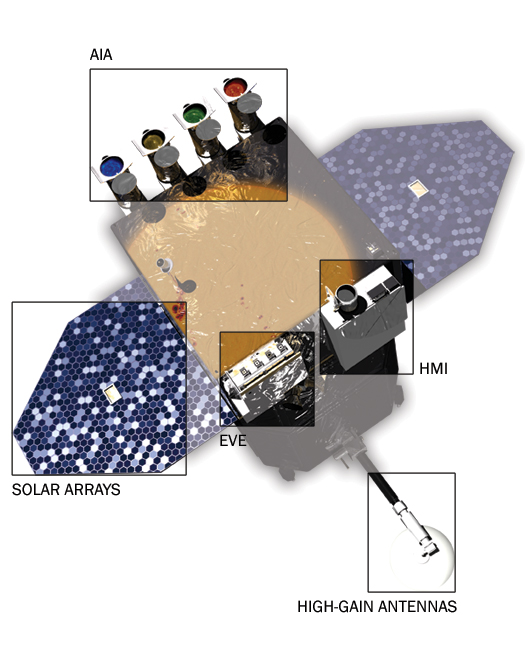
\includegraphics[width=0.5\textwidth]{images/spacecraft_detailed.jpg}
    \caption[SDO Spacecraft]{Solar Dynamics Observatory Spacecraft.
      Image obtained from {\url{https://sdo.gsfc.nasa.gov/mission/spacecraft.php}}}
    \label{fig:sdo_spacecraft}
\end{figure}

We are using Atmosphere Imaging Assembly (AIA) instrument of Solar Dynamics Observatory (SDO; \citep{Pesnell2011})(\cref{fig:sdo_spacecraft}) for the Sun's spectral irradiance data. SDO is a space observatory launched by NASA on 2010 as a part of `Living With a Star' (LWS) program. The spacecraft contains three instruments on board: Extreme Ultraviolet Variability Experiment (EVE), Helioseismic and Magnetic Imager (HMI), Atmospheric Imaging Assembly (AIA). We'll be focusing on the AIA instrument, since that is what we are using. AIA was built in partnership with Lockheed Martin Solar and Astrophysics Laboratory (LMSAL). AIA contains 4 cassegrain telescopes which are optimized to observe narrow bands in the EUV region. Each of the four f/20 telescope has a 20-cm primary mirror and an active secondary mirror. The telescope is designed to prevent charged particles from reaching the Charge Coupled Device (CCD). Field of View (FOV) of each of the telescope is 41 arcmin in circular diameter. The mirrors have special multilayer coatings that are optimized to observe the selected EUV wavelengths of interest. Three of the telescopes have two different EUV bandpasses. The CCDs are back-thinned and back-illuminated with 4096 $\times$ 4096 pixels capturing capabilities. Each of the 12 $\mu$m pixel corresponds to 0.6 arcsec. The telescopes have a selector mechanism to choose the wavelength. AIA captures full-frame EUV image and one UV or visible-light image every 12 seconds. \citep{Lemen2011}\\

\begin{table}[h!]
    \centering
      \setlength{\tabcolsep}{10pt}
      \renewcommand{\arraystretch}{1.5}
    \begin{tabular}{| l | l | l | l |}
      \hline
       \textbf{Band} & \textbf{Primary role, ion(s)} & \textbf{Region of Sun's atmosphere} & \textbf{logT{[}K{]}} \\
      \hline
      4500 Å & Continuum            & Photosphere                                            & 3.7                                   \\
      \hline
      1700 Å & Continumm            & Temperature minimum, photosphere                       & 3.7                                   \\
      \hline
      304 Å  & He II                & Chromosphere, transition region                        & 4.7                                   \\
      \hline
      1600 Å & C IV, continumm      & Transition region, upper photosphere                   & 5.0                                   \\
      \hline
      171 Å  & Fe IX                & Quiet corona, upper transition region                  & 5.8                                   \\
      \hline
      193 Å  & Fe XII, XXIV         & Corona and hot flare plasma                            & 6.1, 7.3                              \\
      \hline
      211 Å  & Fe XIV               & Active region corona                                   & 6.3                                   \\
      \hline
      335 Å  & Fe XVI               & Active region corona                                   & 6.4                                   \\
      \hline
      94 Å   & Fe XVIII             & Flaring regions                                        & 6.8                                   \\
      \hline
      131 Å  & Fe XX, XXIII         & Flaring regions                                        & 7.0, 7.2                              \\
      \hline
    \end{tabular}
    \caption{AIA wavelength channels. Table obtained from \url{https://aia.lmsal.com/public/instrument.htm}}
    \label{tab:aia_wav_channels}
\end{table}

\begin{figure}[h!]
    \begin{subfigure}[b]{0.5\textwidth}
        \centering
        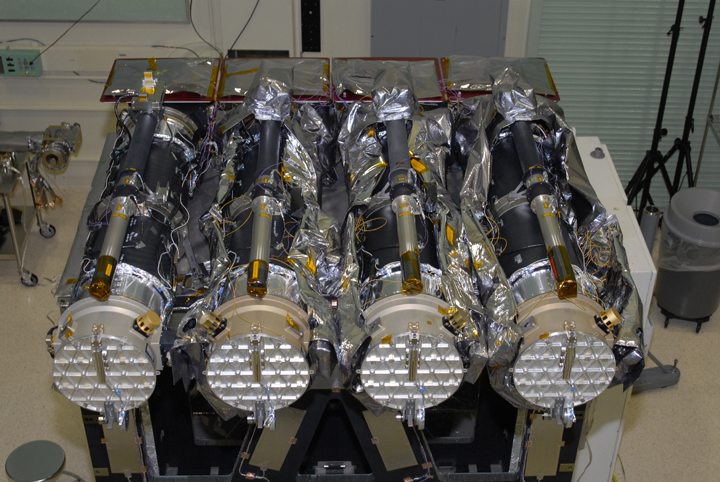
\includegraphics[width=\textwidth]{images/SDO AIA Telescopes.jpg}
        \caption{ }
        \label{fig:aia_telescopes}
    \end{subfigure}
    \hfill
    \begin{subfigure}[b]{0.5\textwidth}
        \centering
        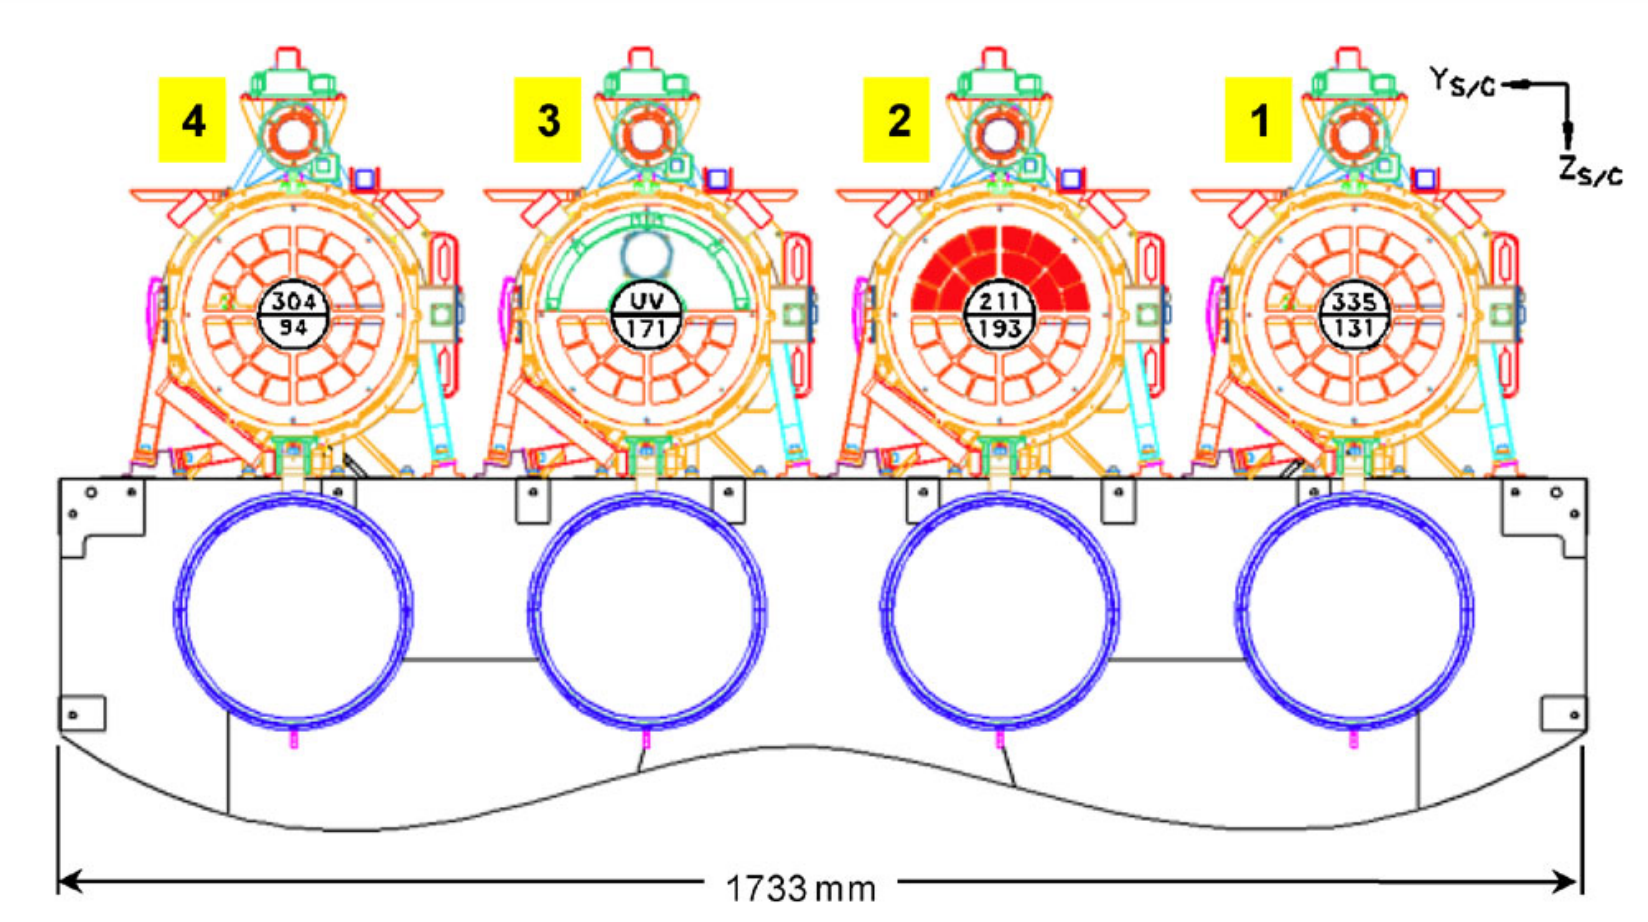
\includegraphics[width=\textwidth]{images/AIA_telescope_layout.png}
        \caption{ }
        {\label{fig:aia_telescope_layout}}
    \end{subfigure}
    \label{fig:aia_telescope_and_layout}
    \caption[AIA telescope and it's Layout]{\Cref{fig:aia_telescopes} shows the AIA telescopes. \Cref{fig:aia_telescope_layout} shows the AIA telescope layout. Telescope 2 has an aperture blade to select between it's two wavelength channels. Rest of the telescopes rely on the filters in filter wheels to select the channel (Image credit: \capcite{Lemen2011})}
\end{figure}

The different channels of AIA respond differently to the radiation of different temperature. The channels of AIA along with it's primary role, region of Sun's atmosphere it probes and temperature has been given in \cref{tab:aia_wav_channels}. The response of the instrument to different wavelengths and temperature is given by it's response curves, which are of two types: \textit{wavelength response curve} and \textit{temperature response curves}. Temperature response curves gives the information about the response of each channel with respect to the temperature of the radiation being received. Temperature response curves play a crucial role in DEM analysis.

\noindent \Cref{fig:aia_tresp} shows the response curves, which has been obtained using \texttt{aia\_get\_response.pro} procedure of SSW IDL.

\begin{figure}[h!]
    \centering
    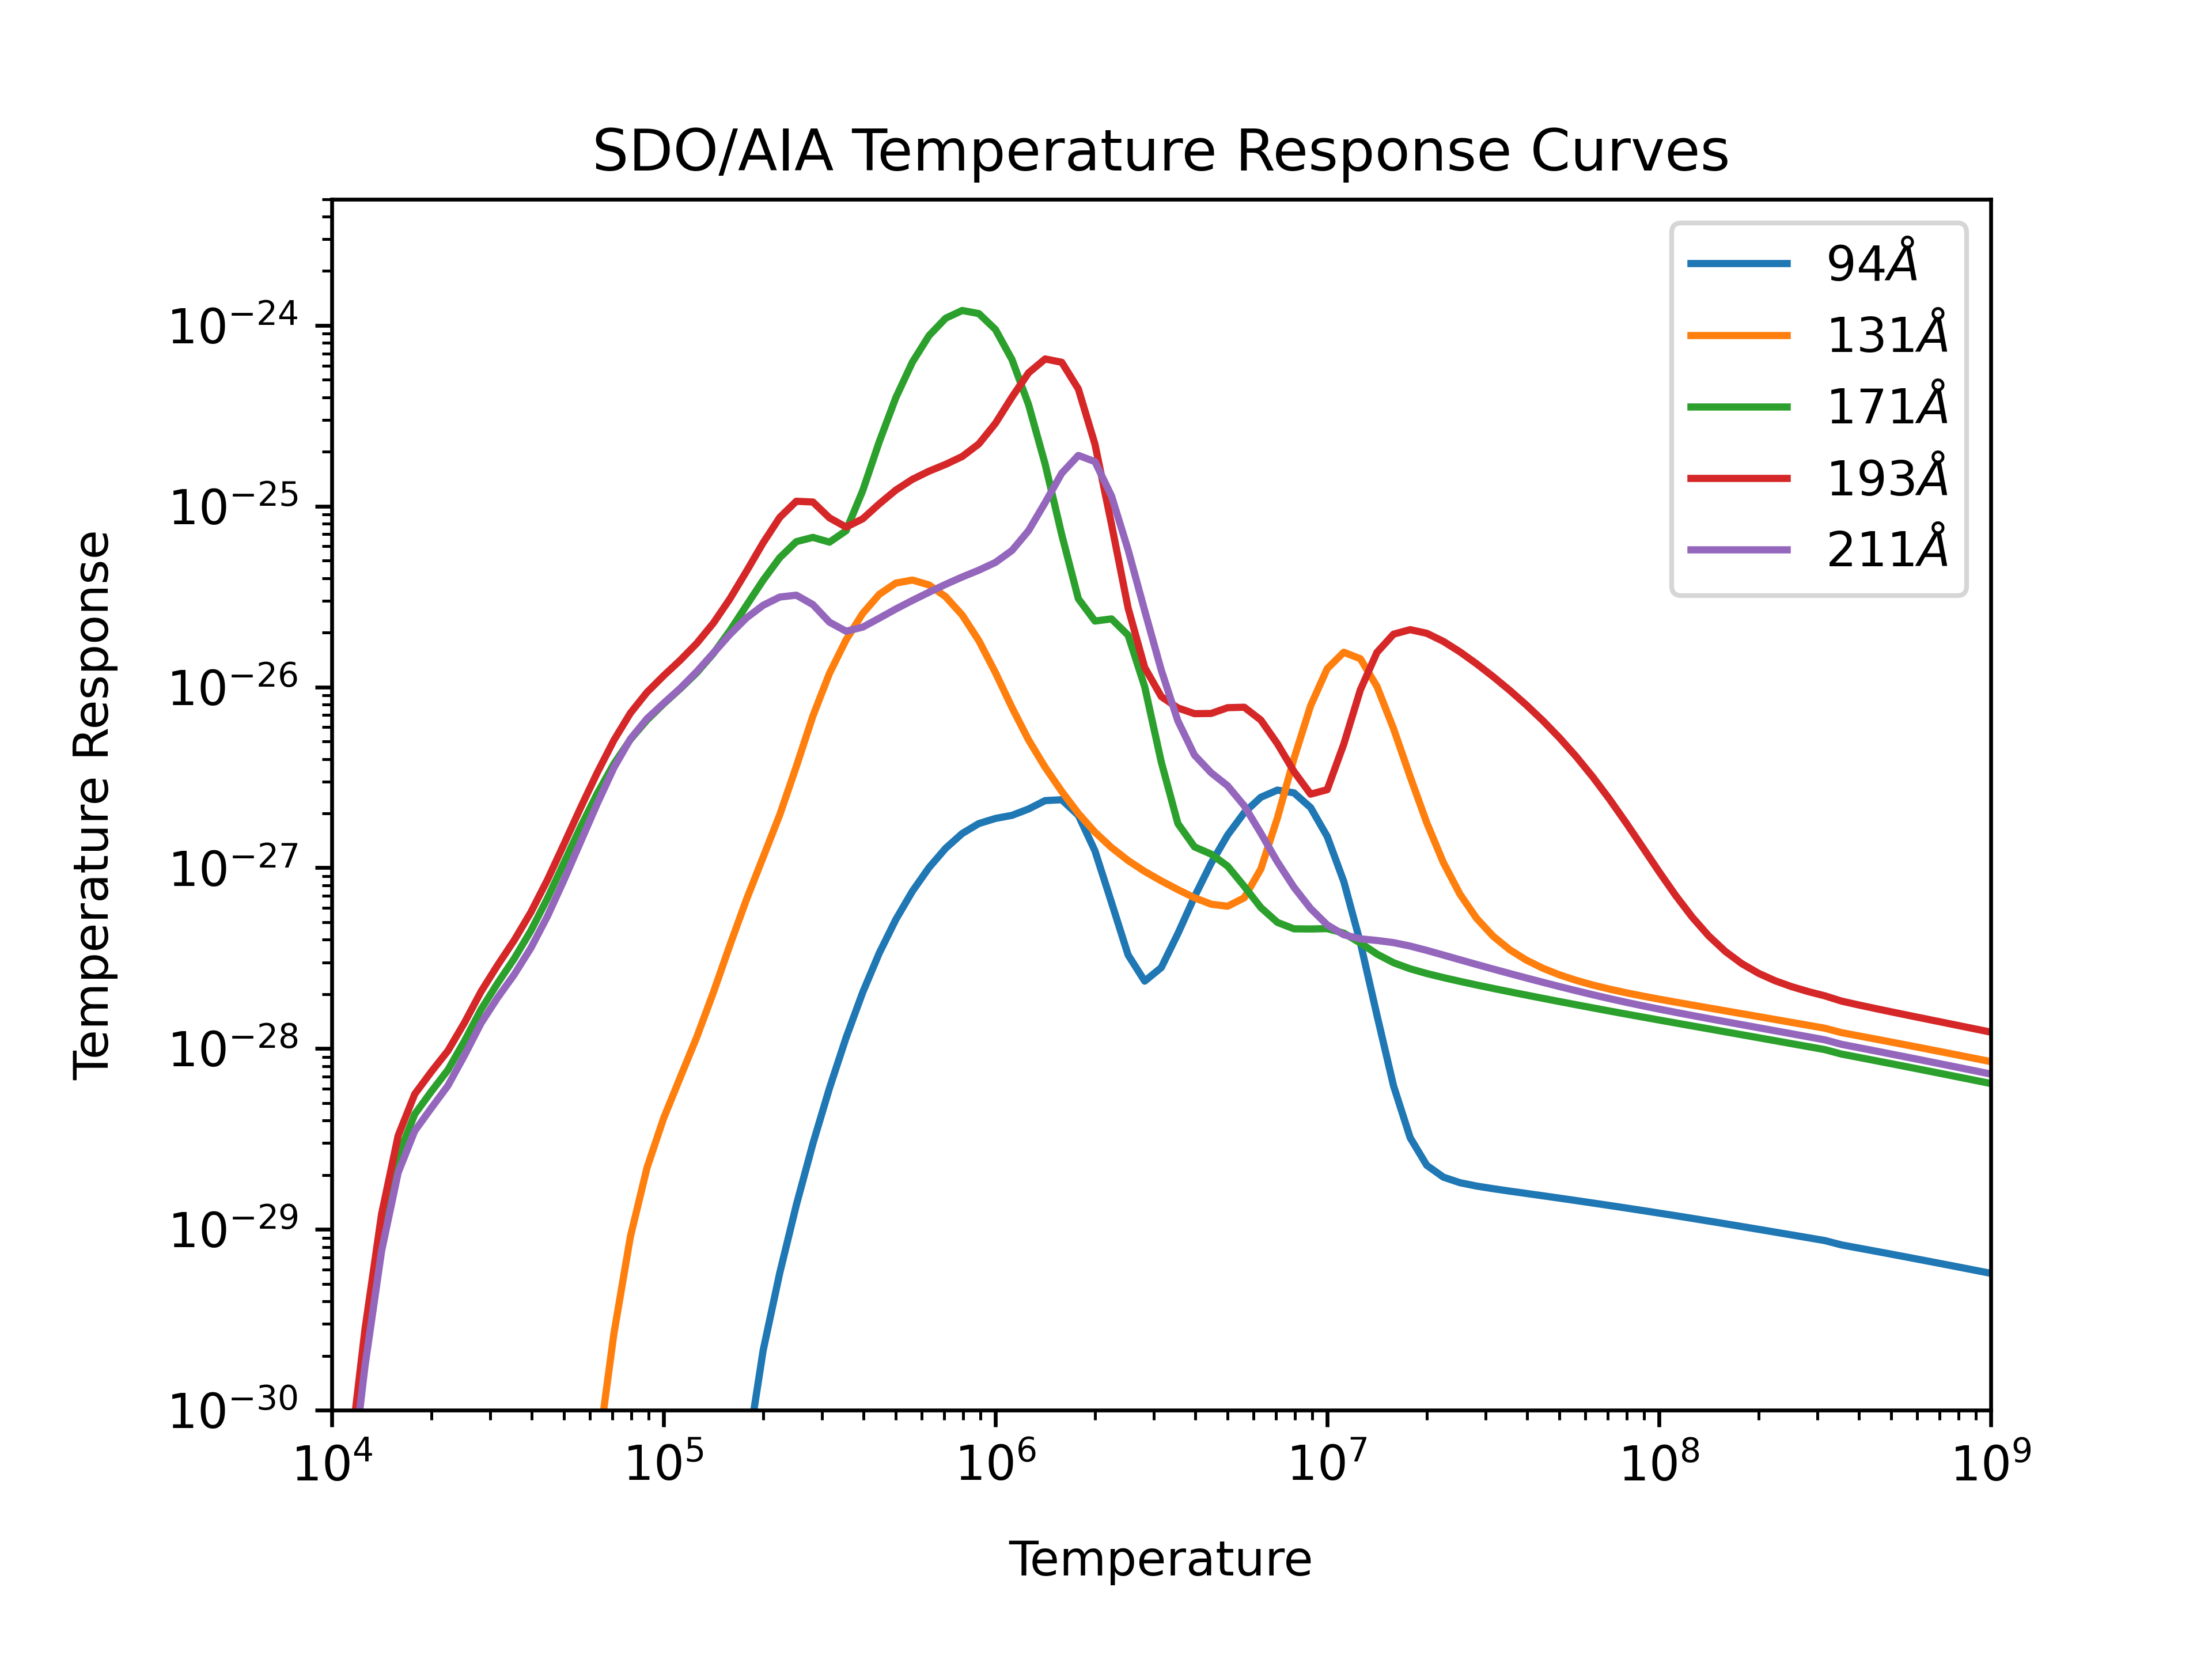
\includegraphics[width=0.75\textwidth]{images/aia_tresp.png}
    \caption[AIA Temperature Response Curves]{SDO/AIA Temperature Response Curves obtained using \texttt{aia\_get\_response.pro}. Curves corresponding to the five wavelength channels required for the DEM analysis has been plotted. Temperature has the unit of Kelvin and temperature response function has the unit of [DN $cm^5 s^{-1} pixel^{-1}$]}
    \label{fig:aia_tresp}
\end{figure}

%%% Local Variables:
%%% mode: LaTeX
%%% TeX-master: "main"
%%% End:
